\documentclass[journal]{IEEEtran}
\usepackage{graphicx}
\usepackage{hyperref}
\usepackage{listings}
\usepackage{xcolor}
\usepackage{media9}
% Path is relative to final_project_report_eantunano.tex
\graphicspath{ {./images/}{../artifacts/docs/circuit_diagrmas/} }


\hypersetup{
  colorlinks,
  linkcolor=blue, % Color of internal links
  urlcolor=blue,  % Color of URLs
  linkbordercolor={1 1 0}, % Yellow border around links
  urlbordercolor={1 1 0} % Yellow border around URLs
}

\begin{document}

    \title{Raspberry Pi 4 Exploration}

    \author{Enrique~Antunano\\University~of~Washington\\enriantu@uw.edu\\{\href{https://github.com/enriquea02/uw/tree/main/eep522a_embedded_and_real-time_systems/submissions/workspace}{https://github.com/enriquea02/uw}}}

    \markboth{EEP522A~Embedded and~Real~Time~Systems, A3~Configuration, February~2025}{}

    \maketitle

    \begin{abstract}
        The scaled back goal of this project was to develop a vector graphic laser display projector that could display a vector image test file with sufficient accuracy that an observer can understand the image that is projected.
        All the supplies, code, schematics, datasheets, and challenges are outlined in this paper, which should be seen as a project description and guide.
        The overall design provides flexibility for miniaturization, wireless control integration, and projection quality improvement, but the current project exceeds a minimal viable product.
    \end{abstract}
    \section{Introduction}
    The intent of this project was to develop a portable vector graphic laser display projector which could take wirelessly uploaded images and project them when commanded to by a user input.
    Quickly, I realized that I did not do sufficient characterization of my project and thus had to scale back significantly from my original goal.
    The new focus of this project was to develop a base laser projector, in only one color, that could draw the International Laser Display Association's (ILDA) test file at the lowest supported speed of 12 kilo point per second (kpps).
    The size, weight, energy consumption, wireless capabilities, and image quality were secondary concerns as the primary goal was to develop a baseline laser projector.

    The scope of this project dealt with challenges in procurement, budget, hardware selection, hardware integration, software testing, and hardware/software integration. 
    The methods, challenges, and results of this project are covered below, but following my paper it should be possible to develop and to continue improving the laser projector project.
    Due to the time constraints of this class, the scope of the project was reduced, but the design is flexible enough for continued tinkering and improvement.

    \section{Methods}

    If starting from a baseline of zero or near zero, then I would block off 50-60 hours for an initial vector laser projector build. 
    The time estimation assumes limited hardware development experience, C/C++ code proficiency, parts selection and procurement, system design, and system integration and test.
    My 40-50 hour projection for the build out is for the whole design cycle. 
    This means from design start till the laser projector is capable of drawing out the ILDA test file.

    Hardware supplies for this project include:
    \begin{itemize}
        \item 15V Dual Power Supply
        \item 2x ILDA Motor Drivers
        \item 2x 15kpps Middle Speed Galvomotors
        \item 5mW Laser
        \item 2x MCP4921 DACs
        \newline Communication via SPI
        \newline 12-bit precision matches DAC code bases found on git
        \item 2x TL082 Dual Channel Op amps
        \item 4x 10k-ohm Potentiameters
        \item Various resistors and capacitors (view schematics linked in Appendices)
        \item Raspbery Pi 4 Model B
    \end{itemize}

    Software for this project include:
    \begin{itemize}
        \item Raspberry Pi OS Bullseye
            \newline SPI enabled through raspi-config
            \newline 2x SPI enabled through /dev/config.txt
        \item WiringPi
        \item ILDA file reader code
    \end{itemize}

    \subsection {Coding Standard}
    This project will use the LLVM Coding Standards. 
    For my decision, I pulled three coding standards: Google C++ Style Guide, LLVM Coding Standards, and Motor Industry Software Reliability Association (MISRA) C/C++.
    MISRA C/C++ will not be used for this projects because it is a purchased standard.
    MISRA's focus is on safety-critical applications, which I think is not applicable for my project.
    Even if my project were safety-critical, there is so little time to develop a working prototype that I care more about readability and consistency than safety-critical applications.
    For a mass-product, which I'll classify as 10,000+ units annually, or human-rated vehicle, then it would make sense to implement a safety-critical coding standard after the prototype phase.
    In my opinion, an engineering development unit would be a good candidate to implement this coding standard.

    I have decided to use the Google C++ Style Guide because it has a better website than the LLVM Coding Standards website.
    The coding standard only applies to new code that I have written for this project.
    It does not apply to source code added to my project from other github repositories.
    Source code will maintain whatever coding standard that it was written with and be used "as-is".
    Easier is entirely subjective. For myself, it is easier to read, navigate, and less verbose.
    The style guide is used for Google open-sourced projects, so it's widely used.
    My focus is on writing prototype code, so I don't want to sit down and read through LLVM Coding Standards right now.
    There may be more merit to the LLVM Coding Standards, but that decision may have to be for another day.

    Click {\href{https://google.github.io/styleguide/cppguide.html}{here}} to be taken to the Google C++ Style Guide.

    \subsection{Hardware Setup}
    This appendix covers the electrical schematics necessary to execute this project.
    Relevant datasheet material will also be included here.

    \subsubsection{Raspberry Pi 4}

    Refer to the schematic listed in Appendix D subsection A for the Raspberry Pi 4 pinout diagram.
    
    Go to the interfaces section to understand the Raspberry Pi 4 pin set up.

    \subsubsection{DAC} 
    
    Refer to Microchip's \emph{MCP4901/4911/4921 8/10/12-Bit Voltage Output Digital-to-Analog Converter with SPI Interface} document listed in the references for the source material.

    The Raspberry Pi 4 drive strength will have to be limited to 2mA to match the DAC's input current electrical characteristics.
    One concern reading the datasheet was that the current at the supply pins were rated to an absolute maximum of 50mA.
    Since the only DACs available, with such short notice on Amazon. were single channel DACs, I needed to purchase two single-channel DACs.
    Each DAC channel drives a single galvomotor. 
    Laser projectors require two galvomotors, one for the X direction and another for the Y direction.
    What concerned me was whether the 5V pins on the Raspberry Pi 4 Model B could supply 100mA (50mA * 2 DACs).
    Reading multiple forums, the current on the 5V rails on the Raspberry Pi 4 are primarily limited by the Raspberry Pi 4 power supply.
    The power supply used in this design is rated for 3.5A, so 100mA is well below that threshold, even accounting for the Raspberry Pi 4's own current draw and any other components. \newline 

    \includegraphics[width=2.5in]{mcp4921_electrical_characteristics.png}

    The gain formula with respect to the reference voltage is listed in the image below. \newline

    \includegraphics[width=2.5in]{mcp4921_gain_formula.png}

    Referring the pinout descriptions below, separate nCS, SCK, and SDI lines will be driven from the Raspberry Pi 4 to the respective X and Y DACs.
    Both DACs will need to be driven simultaneously and I have spare pins on the Raspberry Pi 4, thus each DAC will have their own set of SPI inputs.
    nLDAC will be tied to GND, referenced to the Raspberry Pi 4, since $V_{out}$ control can be set on the rising edge of nCS.
    Tying nLDAC to low also saves the use of two pins on the Raspberry Pi 4.
    $V_{REF}$ will be set to 2.0143V because it is relatively close to the typical 2.038V reference voltage that is listed in the Microchip documentation.
    I can use a simple voltage divider on the 3.3V power rail pins of the Raspberry Pi 4 to get 2.0143V.
    The documentation is unclear whether $V_{DD}$ an $V_{REF}$ need to be related.
    Additionally, it is unclear whether the input SPI pins need to be related to $V_{DD}$ or $V_{REF}$.
    For now, I'm moving forward with the risk since I think it's low.
    The Raspberry Pi 4 has an OCP circuit that I think will protect the Raspberry Pi 4.
    Finally, the voltage divider for $V_{REF}$ uses high resistance vales to limit the current flow to the DAC. \newline

    \includegraphics[width=2.5in]{mcp4921_pin_descriptions.png}

    Final note on the DAC circuit, a bypass capacitor and a high-frequency noise filtering capacitor were placed on the 5V rail as recommended by the datasheet. \newline

    \includegraphics[width=2.5in]{mcp4921_psu_and_dig_intf.png}

    Refer to the schematic listed in Appendix D subsection B for the DAC circuit diagram.
    
    \subsection{ILDA Bipolar Op Amp}

    The ILDA standard specifies that the input voltage to an ILDA motor driver should be $\pm$ 5V.
    The output of the DAC, assuming an ideal of 0V - 3.3V, requires a bipolar op amp to extend the range to $\pm$ 5V.
    The DAC was configured to its max gain output $2 * V_{REF}$, where $V_{REF}$ = 2.0143V as specified in the previous subsection.
    
    Thus, to create the $\pm$ 5V, set up two bipolar op amp circuits.
    One for the x-axis and another for the y-axis.
    In addition to having two bipolar op amps, each bipolar op amp consists of two stages.
    The first stage adjusts the gain, which increases the DAC voltage output from 0V - 3.3V to 0V - 10V.
    Second stage of the bipolar op amp adjusts the offset of the output, moving the 0V - 10V output to -5V to 5V.

    The op amps used for the bipolar op amp circuit is the TL082 op amp, because it is a two-channel op amp which allows for the two stage bipolar op amp to be developed in a compact size.
    A benefit of the op amp is that it can take an input voltage of $\pm$ 2.25V to $\pm$ 20V.
    Please refer to the \emph{TL08xx FET-Input Operational Amplifiers} datasheet for information and the pin out of the op amp. It is linked in the references section.

    First stage consists of an inverting amplifier with a gain of around $G = - \frac{10}{3.3} = -3.03$.
    The resultant DAC output will go from 0V - 3.3V to -10V - 0V.
    Use the following formula to solve for the necessary $R_{f}$ and $R_{i}$ to achieve a gain of -3.03.
    $$ G = -\frac{R_{f}}{R_{i}}$$
    Set the positive input of the first TL082 op amp to ground to keep the first stage easier calculations simple.

    Second stage of the bipolar op amp will consist of an inverting summing amplifier.
    The negative terminal inputs of the summing amplifier consist of the first stage output and an adjustable voltage divider from the positive 15V terminal of the power supply.
    Use the following formula to solve for the necessary resistance values to achieve a negative 5V offset.
    $$ V_{out} = -(\frac{R_{f}}{R_{in}}) * (V1 + V2)$$ 
    Math for the summing amplifier was kept simple by setting all the $R_{in}$ resistors to be equal.
    The negative input of the TL082 op amp was tied to the same ground as the inverting amplifier to keep the math simple.
    Refer to the schematic listed in Appendix D subsection C for the ILDA Bipolar Op Amp circuit diagram.

    \subsection{Interfaces}
    The laser controller requires the following physical interfaces:
    \begin{itemize}
        \item GPIO pin
        \item SPI pins
        \item Power Pins
    \end{itemize}

    Only one GPIO pin was used for this project, BPM GPIO23, which is used to toggle power to the red laser.
    The Raspberry Pi 4 pin out diagram in Appendix D lists GPIO24 and GPIO25 for the green and blue laser diode controls respectively, but those pins are only reserved through documentation.
    The remaining GPIO pins are used for the two DAC SPI interfaces.

    For this project, Raspian's \emph{spidev} Linux utility was used to setup and drive the SPI interfaces from the Raspberry Pi 4. 
    The Linux utility it limited to only two SPI interfaces, which was sufficient for this project.
    Two SPI interfaces are required by this project to drive the two galvo motors.
    One interface will drive the X-axis mirrors while the other will drive the Y-axis mirrors.
    
    Refer to the code below for checking if your system has the \emph{spidev} utility.

    \begin{lstlisting}[frame=single, basicstyle=\ttfamily\footnotesize, breaklines=true]
        ls -la /dev/
    \end{lstlisting}

    Search for a folder named \emph{spidev}.
    There may be numbers as part of the folder name and that's okay.
    Follow the instructions below if the \emph{spidev} folder does not exist.
    If not, read the screenshot below to install the \emph{spidev} library.

    \includegraphics[width=2.5in]{enable_spi_on_rpi4.png}

    Now search for the library again because you should see the following two folders after reboot.

    \includegraphics[width=2.5in]{spi4_installed_after_reboot.png}

    Enabling the SPI setting in the using \emph{raspi\_config} only sets one SPI controller though unfortunately. 
    Although the first SPI controller is enabled, it needs to be modified.
    Additionally, the second SPI pins need to be enabled.
    
    \begin{enumerate}
        \item Copy \emph{config.txt} under /boot to a safe location
        \item Open the text file under the /boot folder with sudo privileges
        
        \begin{lstlisting}[frame=single, basicstyle=\ttfamily\footnotesize, breaklines=true]
            sudo vi /boot/config.txt
        \end{lstlisting}

        \item Find the following line
        
        \begin{lstlisting}[frame=single, basicstyle=\ttfamily\footnotesize, breaklines=true]
            dtparam=spi=on
        \end{lstlisting}

        \item Add the following line underneath, then save and close file
        
        \begin{lstlisting}[frame=single, basicstyle=\ttfamily\footnotesize, breaklines=true]
            dtoverlay=spi0-1cs,no_miso
            dtoverlay=spi1-1cs,cs0_pin=16
        \end{lstlisting}

        \item Now reboot the Raspberry Pi
        
        \begin{lstlisting}[frame=single, basicstyle=\ttfamily\footnotesize, breaklines=true]
            sudo reboot
        \end{lstlisting}

        \item View /boot/config.txt to verify the modification highlighted
        \item List everything under the /dev folder and verify that \emph{spidev1.0} is now listed alongside \emph{spidev0.0} and \emph{spidev0.1}
    \end{enumerate}

    Finally, one 3.3V, 5V, and GND pin of the Raspberry Pi 4 are connected to the DAC and ILDA Bipolar Op Amp driver circuits. 
    The 3.3V is used to drive the DAC $V_{REF}$ input, the 5V DAC power rail, and common ground is connected between the 15V power supply and the Raspberry Pi 4.

    \subsection{Code}

    As for code, the code base can roughly be outlined with the following diagram.

    \includegraphics[width=2.5in]{system_level_architecture_diagram.png}

    All code pulled from other git users, included in the references, did not have the Google C++ style guide apply to them.
    Rather, code from other users was grandfathered in, with only minimal modifications made when necessary.
    Code that I developed did attempt to conform to the Google C++ style guide.

    The motor drivers were pulled from github user \emph{tteskac}, github project \emph{rpi\_lasershow}.
    The motor driver uses a library developed by ABElectronics, which translates decimal inputs between 0-4095 into SPI commands which are then driven to the DAC.
    The SPI commands are sent using IOCTL.
    Code for the motor driver also activates and closes the DAC.
    In contrast, the laser driver code is very straightforward and easy to implement using the WiringPi library

    Looking at the next level of abstraction, the image and command sequencers were covered by the ILDA reader developed by \emph{tteskac}.
    The ILDA reader follows the ILDA Format 5 - 2D with True Color.
    The ILDA format consists of a 32 byte header, x/y/z motor commands, laser on/off commands, and red/blue/green light intensity information.
    Each ILDA packet covers information for a single laser point and consists of 8 data bytes.

    \includegraphics[width=2.5in]{ilda_command_packet.png}

    All the code I listed is contained in a git submodule, linked to \emph{tteskac}'s \emph{rpi\_lasershow}. 
    The \emph{rpi\_lasershow} directory contains a subfolder called \emph{ilda\_files} which contains the \emph{.ild} files which would be projected by my laser projector

    The two pieces of code that I developed were first, the "glue" logic that managed the ILDA reader and motor drivers.
    Refer to github link at the top of this then go to the following file \emph{src/laser\_proj\_top.cc} which contains all the glue logic.

    Then for testing, I wrote \emph{src/motor\_drvr\_lib.cc} which is used to generate a sine wave from the DAC minimum (0V) to the DAC maximum (3.3V).
    This code allowed for validation and calibration of the motor driver signal from the Raspberry Pi 4 edge through the DAC and Bipolar Op Amp supply, up to the edge of the motor driver card.
    Although I could have used the github code + my glue logic to do the same validation, developing a motor driver test script allowed for calibration of the bipolar op amp's \emph{gain} and \emph{offset} to achieve the ILDA $\pm$ 5V standard input. 

    The motor driver test code and the laser projector code can both be compiled using the Makefile I developed.

    To create a motor driver test executable, type the following command into the terminal window while in the \emph{src} directory.
    A file called \emph{../bld/motor\_driver} will be generated after the make command is run on the raspberry pi 4.

    \begin{lstlisting}[frame=single, basicstyle=\ttfamily\footnotesize, breaklines=true]
        make clean
        make motor_driver
    \end{lstlisting}

    To create a laser projector executable, type the following command into the terminal window while in the \emph{src} directory.
    A file called \emph{../bld/laser\_projector\_top} will be generated after the make command is run on the raspberry pi 4.

    \begin{lstlisting}[frame=single, basicstyle=\ttfamily\footnotesize, breaklines=true]
        make clean
        make
    \end{lstlisting}

    To run the laser projector code after compiling and building the code, type the following commands from the \emph{bld} directory.
    The code will run indefinitely until \emph{ctrl+C} is entered into the SSH terminal window, which connects the host machine to the Raspberry Pi 4. 

    \begin{lstlisting}[frame=single, basicstyle=\ttfamily\footnotesize, breaklines=true]
        ./laser\_projector\_top [time between laser firings] [.ild file path and name]
    \end{lstlisting}

    An example launch command is shown below, assuming the executable is launched from the \emph{bld} directory.

    \begin{lstlisting}[frame=single, basicstyle=\ttfamily\footnotesize, breaklines=true]
        ./laser\_projector\_top 0 ../src/rpi\-lasershow/ilda\-files/test.ild
    \end{lstlisting}

    \section{Results}
    \subsection{Hardware Setup}
    This subsection covers the results from hardware setup.

    \subsubsection{Raspberry Pi 4}

    For the Raspberry Pi 4, integration of the Raspberry Pi 4 GPIO and power pins the circuit did not have any notable results.
    An app, RaspController, was used to test the power toggle of the laser diode. 
    The app allows for easy SSHing into the device and discrete toggling of each GPIO pin on the device.
    Go to Appendix B for instructions on how to download and set up the RaspController app on your mobile phone. 

    \subsubsection{DAC}

    To validate DAC set up, $V_{REF}$ was measured to be 2.0148V.
    The measurement was taken across the 3.3V voltage divider with respect to the Raspberry Pi 4 ground.
    After setting up the DAC, the max output voltage was measured with a multimeter to be roughly 3.1V rather than 3.3V. 
    The minimum voltage output of the DAC was 75mV.
    Neither the maximum nor the minimum output voltages were values that I expected, but the imperfections could be dealt with through the bipolar op amp circuit.

    \subsubsection{ILDA Bipolar Op Amp}
    For the DAC output, I was only able to achieve a voltage range of 0V - 3.1V with a precision of $\frac{1}{4096}$ from the 12-bit DAC output, as measured by a multimeter.
    Using the first stage of the bipolar op amp, the voltage output range stretched from 75mV to -10.013V as measured by the multimeter.
    The second stage, the summing amplifier, created a voltage output ranging from -4.930V to 5.013V for the X galvomotors input, and a similar value for the Y gavlometer input.
    The gain and offset potentiameters allowed for both bipolar op amp outputs, the X and Y galvomotors outputs, to be tuned to meet the $\pm$ 5V output.
    Differences from the DACs and resistance values could only be corrected for by the gain and offset potentiameters.

    \subsection{Integrated Laser Projector}
    
    An image of the integrated laser projector is provided below.

    Starting from the top-right and going clockwise, the first component is the Raspberry Pi 4 Model B.
    Connected to the DAC circuit, which is then connected to the ILDA bipolar op amp circuit on the same breadboard.
    Then the breadboard is connected to the laser diode.
    Bottom-left are the X and Y galvomotors.
    Motor drivers for the galvomotors are connected directly above. 
    Finally, the DC power supply is connected to the ILDA bipolar circuit on the breadboard and motor driver board.

    \includegraphics[width=2.5in]{prototype_hw_setup.png}

    Now most importantly, I have included an image of the vector laser projector output when running the \emph{test.ild} file

    \includegraphics[width=2.5in]{vector_laser_projector_image.png}

    \includegraphics[width=2.5in]{vector_laser_projector_image2.png}

    \includegraphics[width=2.5in]{vector_laser_projector_image3.png}

    \section{Discussion}
    \subsection{Laser Projection}
    
    Although I'm very impressed with myself for selecting the hardware, integrating the components, tuning the hardware, developing the top-level "glue" code and test code, there is a still a large amount of room for improvement in this project.
    I was far outside my wheelhouse initially, but now I know where I fell short in my characterization, what could have been improved, and the best next steps to improve my project in the future.

    First, observing the laser projection.
    On a first prototype baseline, I was impressed that the quality of the laser output was sufficient.
    If reviewing the laser image from the results tab above, you can see that it's relatively faithful to the ILDA's test image.

    \includegraphics[width=2.5in]{ilda_test_image_key.png}

    All the flaws of the current image projector will reference the ILDA Test Image Key.
    First, the current projector has trouble reproducing circles, which likely results from DACs X and Y being slightly out-of-sync.
    For future iterations, I would connect the nLDAC pins of both DACs to a single Raspberry Pi 4 GPIO pin, that way the two single-channel DAC outputs can be launched synchronously.
    From a hardware standpoint, it was much easier to tie both nLDAC pins to ground, so I wouldn't have to write code to manage the synchronization of both the X and Y DAC outputs.
    At the time of my project characterization and exploration phase, I did not consider that I'd need DACs to feed inputs to the motor driver board, so it felt rushed to read through the datasheets of the MCP4921 DACs and TL082 Op Amps.
    So in the future, I'd dedicate more time to figuring out what hardware I'd need and highlighting common features amongst different part vendors, so that I can develop a better generic module that has features such a synchronous output latching already included.
    This would allow me to be more hardware-agnostic in the future, as opposed to now where my Raspberry Pi 4 code is targeted for the Microchip DAC family.
    
    Another point of failure in my current design is that the projector is struggling to create fine points of various intensity as seen in image 2, tying to B3/B4.
    From the ILDA Test Pattern Key, this issue can also be solved through tying the nLDACs together and also better aligning the bipolar op amp offset potentiameters to use the whole $\pm$ 5V range. 

    The final image shows that the laser projector is excellent at centering as the edges of the squares are well aligned and clearly distinct.
    The X and Y letters are inverted though, which can be easily corrected in hardware or software by flipping the outputs.

    \subsection{Laser Projection Code}
    
    Vector laser projectors use an industry standard file format, set by the \emph{International Laser Display Association}, to convert images and videos into a laser display.
    Files are saved with the \emph{.ild} file handle.
    The file describes the X-Y commands and laser ON/OFF sequences which drive the mirror motors and laser diode respectively.

    There is software, such as Laserworld's \emph{Showeditor}, that can export files into a \emph{.ild} format.
    This project avoids the use of commercial software, such as \emph{Showeditor} for two reasons.
    First, their free tiers, if available at all, have very limited functionality.
    My research indicates that the free-tier from \emph{Showeditor} is sufficient for simple \emph{.ila} file exporting. 
    Any additional features will require a professional license though.
    For hobbyist purposes, \emph{Showeditor} seems like the only/best option.
    Second, my primary workstation only has Linux installed and the free-tier of \emph{Showeditor} only supports up to Windows Vista.
    Although I could install a VM or a dual-boot system, I would rather avoid installing an old version of Windows for the use of running one software package.
    As a final statement, I did try to run Showeditor using \emph{Wine} on my Ubuntu-based Linux machine, but \emph{Showeditor} failed to boot.

    Due to the issues highlighted, I found a workaround. 
    The github user, \emph{marcan}, has developed a {\href{https://github.com/marcan/openlase/blob/master/tools/svg2ild.py}{script}} that converts \emph{.svg} file types into \emph{.ild} file types.
    There are known bugs and issues with the script, code inefficiencies and possible missing RGB support, but as a development project those issues are fine. 
    My current project only works with one light source, red, so possible missing RGB support is not an issue.
    Plus, I have found another user who has implemented \emph{marcan's svg2ild.py} script onto a Raspberry Pi Zero and has a functional laser projector.
    Click {\href{https://github.com/phuid/laser_projector?tab=readme-ov-file#hw}{here}} to be taken to the github page of \emph{phuid}, who has implemented the \emph{svg2ild.py} script for use in their Raspberry Pi Zero.
    Since the project has been implemented by another user on a more resource constrained Raspberry Pi Zero, I am not worried about code inefficiencies with the \emph{svg2ild.py} script.
    
    For now, the svg2ild conversion is not included, but this does highlight large "misses" during the characterization stage of my project.

    To create a laser animation using a \emph{.svg} file, go to appendix \emph{Create Laser Animation}.

    \subsection{Discrete Electronics}
    Sourcing parts on a short notice, 3-5 weeks prior to March 17th, presented challenges with lead times.
    Long lead times forced me to substitute parts, such as a single dual-channel DAC with two single-channel DACs to drive the X and Y galvomotors respectively.
    Also, the long lead times not only limited my selection of parts, but limited where I could purchase those parts at such low volumes.

    Amazon was the best option due to their return policy, delivery speed, and having at least one option/substitute electronic component available.
    The drawbacks of using Amazon were, first, it was more expensive for equal or lower quality parts compared to vendors such as Digikey, Avnet, or AliExpress.
    Many online writers of at-home vector laser projectors sourced cheap parts from AliExpress, but none mentioned the long lead times for the components.
    The second drawback of Amazon was that many parts had sparse electrical characteristic documentation.
    I searched Amazon, Alibaba, and Ebay to find documentation on the motor drivers and the galvomotors, but nome existed.
    Thankfully, the motor driver came with a test laser output board.
    I used the test board to verify that the galvomotors and motor driver cards functioned correctly, and to verify that expected input into the motor driver board.
    For example, I tried to drive the motor driver using my motor driver code, but the motor driver board expects the ILDA header before forwarding the motor commands to the two galvomotors.

    For this project, before I switched from a stepper motor to a galvomotor, I was interested in the stepper motor selection on Digikey because they were better documented and were more precise. 
    Ultimately, I went with a stepper motor on Amazon that lacked documentation because the motor would arrive faster and the motor was 50\% cheaper. 
    One example was when I purchased a motor driver circuit from Amazon.
    The vendor had no workable documentation on their Amazon page, such as a pin out diagram.
    Before switching from a stepper motor to a galvomotor, which made the motor driver irrelevant for my project, I had to look up the datasheet of the TI DRV8825 microcontroller that was on the PCBA and assume all the datasheet information was still applicable.

    In continuation, the wish I spent more time on motor selection and motor driver file types during the Assignment 2 characterization. 
    I bought stepper motors and galvomotors because I wasn't sure which path was best for my project.  
    Quickly, I realized that stepper motors required potentiameters to align/zero themselves.
    Additionally, stepper motors are suited for laser engraving/CNC milling purposes.
    So the file type best suited for stepper motors is a CNC milling file type that has information such as \emph{step count} in the file data packet, which are not available in the \emph{.ild} file type.
    There was also much more material and better suited material for galvomotors, since the \emph{.ild} file type was written for galvomotors in mind.
    From an integration speed and ease-of-use view, galvomotors were the better choice, but at a higher cost.
    All of this information could have come out during the characterization phase, but these issues did not cross my mind at the time.

    Another challenge that I faced was with handling substitute parts. 
    After extensive research, I found a set of vector laser projects that were well documented and were complete enough for me to use and implement in such a short period of time.
    Due to the time crunch of this project, I had to use substitute parts from the source documentation.
    The new parts forced me to do circuit modifications, write code to target different microcontrollers, and do additional research to verify that the Raspberry Pi 4 had enough pins and that I wouldn't fry the Raspberry Pi 4 when hooking up the substitute components.
    For this project, I had to substitute:
    \begin{itemize}
        \item Dual-channel DAC for two single-channel DACs
        \item XY Galvo-motors and motor driver boards
        \item Arduino with a Raspberry Pi 4
    \end{itemize} 

    The biggest pain was the substitute of the Dual-channel DAC for the two single-channel DACs. 
    The DACs are not as well in-sync as a single chip dual-channel DAC.
    The \emph{ABElectronic} code that I pulled was written for the dual-channel DACs, so the driver code had to be modified to drive the two DACs separately.
    Due to the timetable of this project, I dropped the more elegant single SPI interface solution, which would've used the chip-selects to communicate with DAC-X and DAC-Y separately.
    Implementation of the single SPI interface may not be difficult, but I was not sure how time-multiplexing the SPI bus would work.
    With most of the pins still free and a whole second set of Linux utility controlled SPI interface pins, I went with using both SPI interface resources.
    From an implementation standpoint, this is easier since I can drive both buses simultaneously without having to deal with a time-multiplexing solution that would still allow the X and Y mirrors to move in-sync.

    \subsection{Wireless Communication}
    My characterization focused on memory usage, pin library tradeoffs, and memory access times.
    Throughout my project, the only thing in my initial characterization that was helpful was the pin library tradeoff.
    In hindsight, I should have looked at hardware early, read datasheets early, and read more into wireless communication so that I can remotely control my projector and drop new images remotely.
    The wireless aspect of my project ended up being throw out because I needed to focus entirely on a baseline prototype projector that could be upgraded in the future.
    That being said, from my latest research, which I failed to collect during the characterization phase, I think I can easily control my laser projector remotely using the RaspController app.

    Using the app, I can SSH into the Raspberry Pi using my phone and launch the laser projector executable. 
    Additionally, I can transfer files from my phone into the Raspberry Pi 4.
    Assuming I have \emph{.ild} files on my phone, I can transfer the file into the Raspberry Pi 4 and log into an SSH session so that I can run my laser projector executable remotely as long as I'm on the same network as the Raspberry Pi 4.
    It's not the file path transfer I intended, but it is an easy way to remotely control the projector and drop new images for it to project. 
    Appendix B has information on downloading and setting up the RaspController app.
     
    \section{Conclusion}

    In reference to my revised project goal of developing a laser projector that can print a simple image, I think I met and exceeded my expectations.
    The laser projector has some trouble tracing out images, but for the most part it can project the test ILDA file well with room for improvement.
    From my exploration of remote-access tools available for the Raspberry Pi, I can wirelessly SSH into the Raspberry Pi 4 using my phone.
    This effectively allows me to transfer files wirelessly and launch/abort the laser controller when I see fit.
    Thus, I think I exceeded my initial goal of developing a laser projector.
    Through the course of this project, I realized that my characterization lacked a lot of detail.
    It failed to identify the best hardware, focused on the wrong things (for example memory usage on a Raspberry Pi 4, which was sufficiently large), and I didn't read through vendor documentation early.
    Throughout this project, size, weight, energy consumption, wireless capabilities, and image quality were secondary concerns as the primary goal was to develop a baseline laser projector.
    In developing a final product, I dealt with challenges in procurement, budget, hardware selection, hardware integration, software testing, and hardware/software integration. 
    Due to the time constraints of this class, the scope of the project was reduced, but the design is flexible enough for continued tinkering and improvement.
    Overall, it was a great project I intend to continue developing.

    \nocite{*}
    \newpage

    \bibliographystyle{ieeetr}
    \bibliography{final_project.bib}

    \newpage
    \section{Acknowledgements}
    The author would like to acknowledge the \emph{WiringPi} team for their GPIO access library for Raspberry Pi boards. \newline

    The author would like to acknowledge the \emph{RaspController} team for their remote access mobile application for Raspberry Pi boards.

    The author would like to acknowledge {\href{https://www.circuit-diagram.org/editor/}{Circuit Diagram}} for their free circuit design software. 

    \newpage
    \appendices
    \section{Download WiringPi Library}
    The library can be built on the device or a prebuilt library can be used. 
    For the Raspberry Pi 4 Model B using the Bullseye Debian in this project, the latest library in the WiringPi GitHub ({\href{https://github.com/WiringPi/WiringPi/releases/tag/3.14}{Release 3.14}}) will be used.

    In a Raspberry Pi SSH terminal, follow the code below to build the WiringPi library.
    \begin{lstlisting}[frame=single, basicstyle=\ttfamily\footnotesize, breaklines=true]
        # fetch the source
        sudo apt install git
        git clone https://github.com/WiringPi/WiringPi.git
        cd WiringPi

        # build the package
        ./build debian
        mv debian-template/wiringpi_3.14_armhf.deb .

        # install it
        sudo apt install ./wiringpi_3.14_armhf.deb
    \end{lstlisting}

    WiringPi was installed in the \emph{\$HOME} directory. 
    If the WiringPi library is installed in a different location in your Raspberry Pi system, then update laser controller scripts to reflect the location of the WiringPi library in your system.

    \section{Setup RaspController Mobile Application}
    \emph{RaspController} is an \emph{iOS} app that allows for easy SSH access into your local Raspberry Pi 4 device.
    The \emph{RaspController} mobile app will be used to control the laser projector manually or drop new laser projection files into the Raspberry Pi 4 device.
    Unless port-fowarding is enabled, your mobile phone and Raspberry Pi 4 device must be on the same network, as this can be treated as any other SSH connection.

    As a future improvement for mass-production, this process should be changed to be more user-friendly, simpler, and less powerful for a regular user.
    At the moment, since the user is SSH-ing into the Raspberry Pi 4 operating system, there's a significant amount of room for error if the user does not know what they are doing.
    My suggestion for making this feature more user-friendly would be to file share via Bluetooth instead.
    For small-volume production, this is an easy path forward and reduces the complexity to the end-user and the risk that the user causes an error.
    As a prototype project though, having full control via a phone is very helpful for development.
    
    Follow the steps below for downloading and connecting to your Raspberry Pi 4 device:
    \begin{enumerate}
        \item Go to the app store, search for \emph{RaspController}, and download the application
        
        \item Navigate through Apple's privacy settings
        
        \item Open the RaspController app and select \emph{Add Device} 
        
        \item Fill in Raspberry Pi 4 device information in the \emph{Add Device} screen
        
        \includegraphics[width=2.5in]{add_device_raspcontroller_app.PNG}
        
        \item Select the added device
        
        \item Ran linux command to test SSH connection
        
        \begin{lstlisting}[frame=single, basicstyle=\ttfamily\footnotesize, breaklines=true]
            ifconfig
        \end{lstlisting}

        \includegraphics[width=2.5in]{ssh_shell_raspcontroller_app.PNG}
    \end{enumerate}

    \section{Create Laser Animation}
    To create a source \emph{.svg} file, which will be converted to a \emph{.ila} file format within the Raspberry Pi 4, follow the guide below.

    Required Software:
    \begin{itemize}
        \item Blender 4.2 or newer
        \item Blender Add-on: Render: {\href{https://extensions.blender.org/add-ons/freestyle-svg-exporter/}{\emph{Freestyle SVG Exporter}}}
    \end{itemize} 

    Blender was selected because it is an open-source, free animation software that is available across most operating systems (Windows, MacOS, Linux).
    The Blender community is fairly large, so there is a sufficient amount of community support.
    The following {\href{https://youtu.be/PrlK5Y74sR8?si=fridcX0fLfz2cV0W}{YouTube}} video was used as a reference to understand how to generate \emph{.svg} file types. 

    \begin{enumerate}
        \item Download Blender software
        \item Download Freestyle SVG Exporter
        \item Follow on-screen instructions for download and select to enable the extension
        \item Follow YouTube video highlighted above for generating a \emph{.svg} file type, except change frame rate to 24fps
        \item The \emph{.svg} file will be generated in the output folder location that was specified 
    \end{enumerate}

    Use this YouTube video, {\href{https://youtu.be/CBJp82tlR3M?si=AnMmnkilE5h2m_C9}{Animation for Beginners}}, to generate an animation for the laser projector.

    \section{Hardware Setup}
    \subsection{Raspberry Pi 4}

    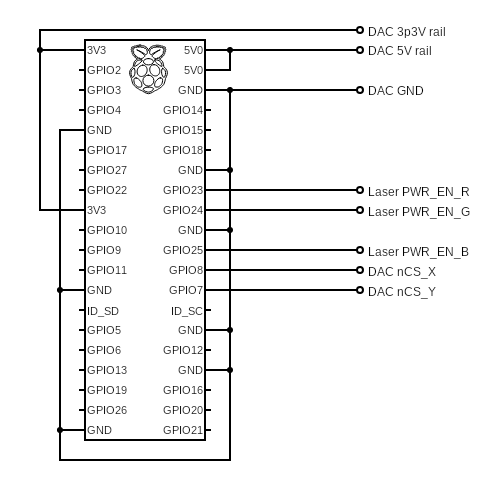
\includegraphics[width=2.5in]{../artifacts/docs/circuit_diagrams/rpi4_circuit.png}

    \subsection{DAC}

    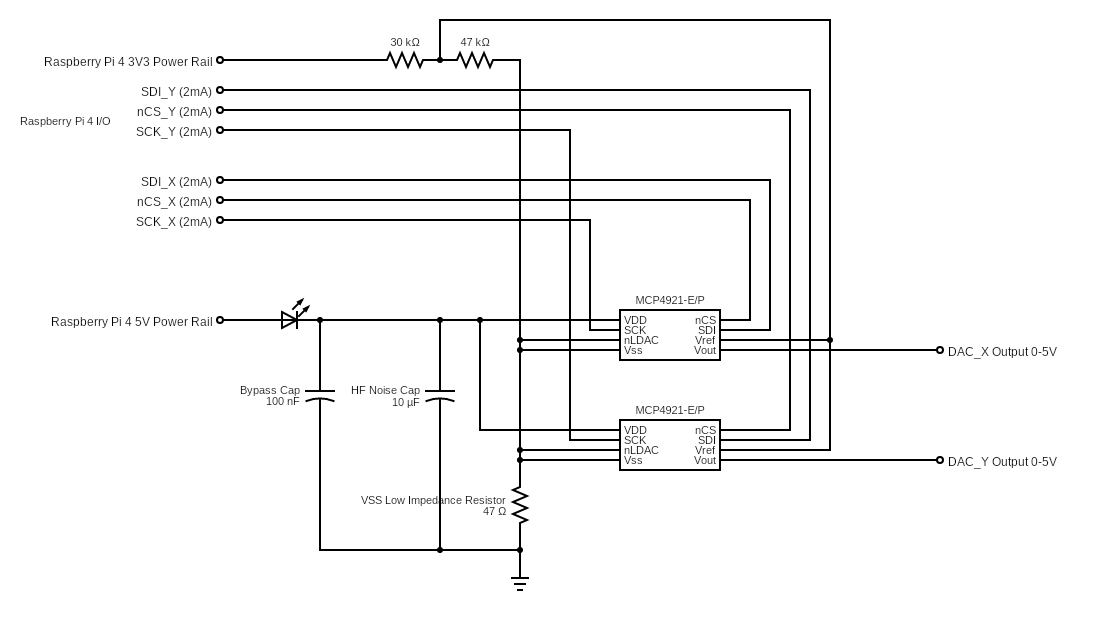
\includegraphics[width=2.5in]{../artifacts/docs/circuit_diagrams/dac_circuit.png}

    \subsection{ILDA Bipolar Op Amp}

    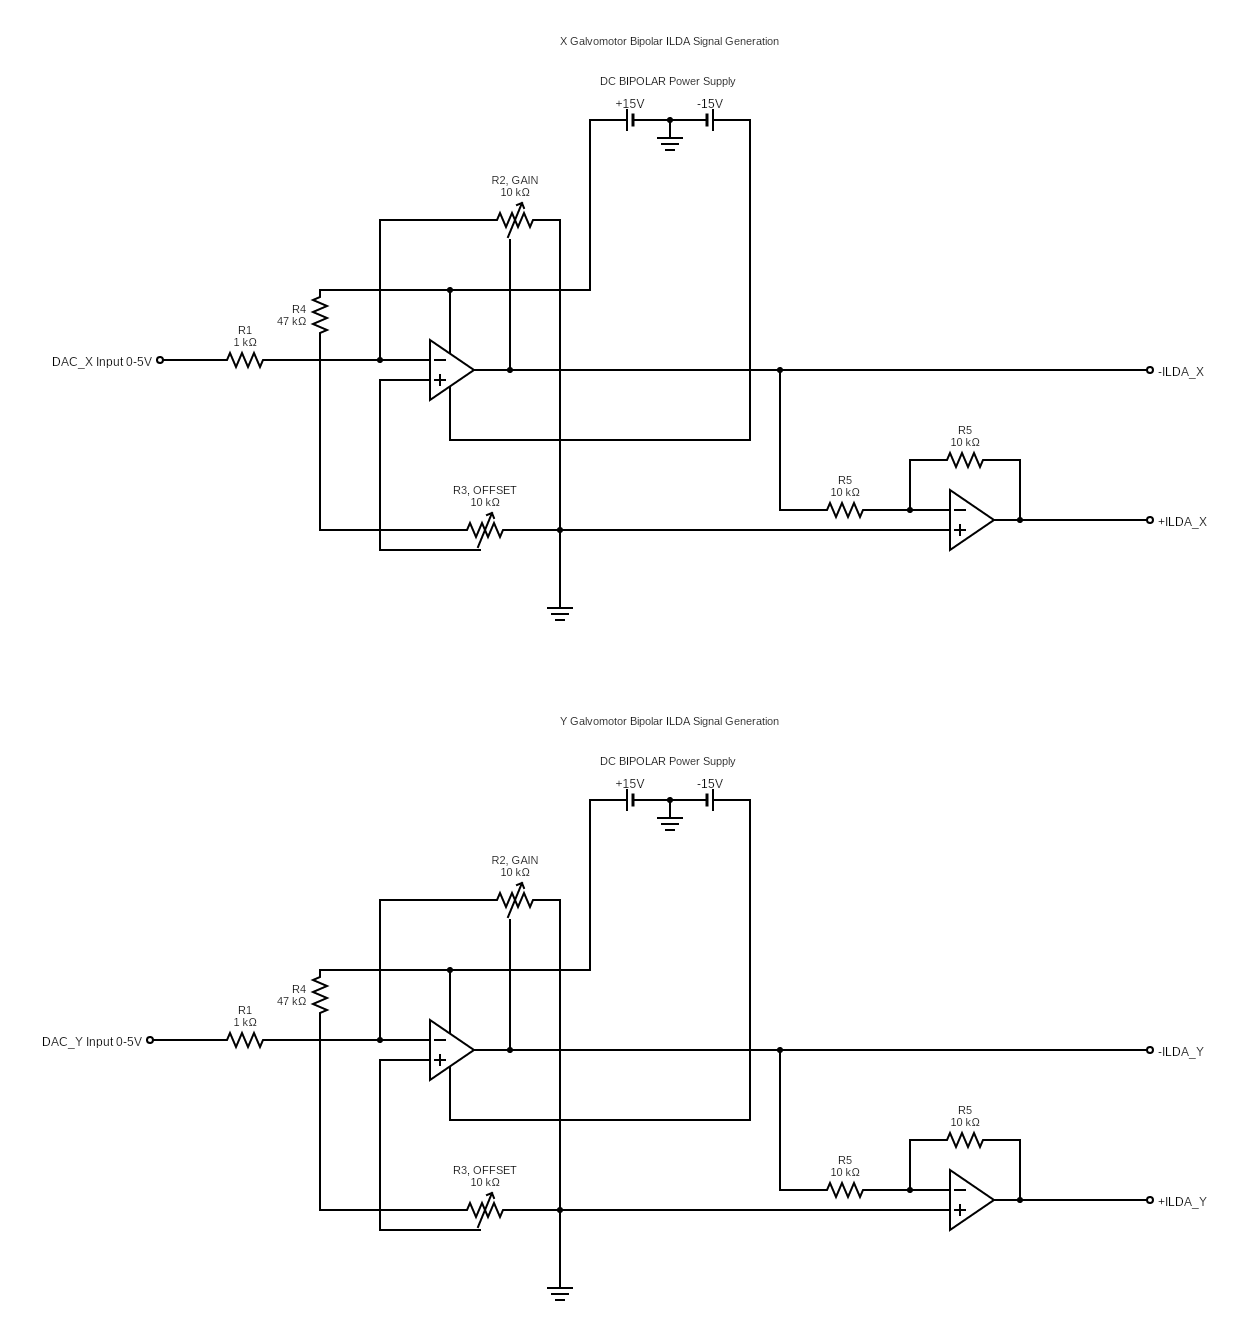
\includegraphics[width=2.5in]{../artifacts/docs/circuit_diagrams/ilda_op_amp_circuit.png}

    \section{Interfaces}
    \subsection{Raspberry Pi 4 SPI Pinout}

    \includegraphics[width=2.5in]{rpi4_spi_pinout.png}

\end{document}